\documentclass[twoside,11pt]{article}

\usepackage{jmlr2e}
\usepackage{listings}
\usepackage{color}
 
\definecolor{codegreen}{rgb}{0,0.6,0}
\definecolor{codegray}{rgb}{0.5,0.5,0.5}
\definecolor{codepurple}{rgb}{0.58,0,0.82}
\definecolor{backcolour}{rgb}{0.95,0.95,0.92}
 
\lstdefinestyle{mystyle}{
    backgroundcolor=\color{backcolour},   
    commentstyle=\color{codegreen},
    keywordstyle=\color{magenta},
    numberstyle=\tiny\color{codegray},
    stringstyle=\color{codepurple},
    basicstyle=\footnotesize,
    breakatwhitespace=false,         
    breaklines=true,                 
    captionpos=b,                    
    keepspaces=true,                 
    numbers=left,                    
    numbersep=5pt,                  
    showspaces=false,                
    showstringspaces=false,
    showtabs=false,                  
    tabsize=2
}
 
\lstset{style=mystyle}

% Heading arguments are {volume}{year}{pages}{submitted}{published}{author-full-names}
\jmlrheading{7}{2016}{1-5}{7/16}{-}{Guillaume Lema\^itre, Fernando Nogueira, and Dayvid V. R. Oliveira}

% Short headings should be running head and authors last names
\ShortHeadings{A python toolbox to tackle the curse of imbalanced datasets in machine learning}{Lema\^itre, Nogueira, and Victor}
\firstpageno{1}

\begin{document}

\title{A python toolbox to tackle the curse of imbalanced datasets in machine learning}
\author{Guillaume Lema\^itre \email g.lemaitre58@gmail.com \\ 
    \addr{LE2I UMR6306, CNRS, Arts et M\'etiers, Universit\'e Bourgogne Franche-Comt\'e} \\ 
    \addr{12 rue de la Fonderie, 71200 Le Creusot, France} \\ 
    \addr{ViCOROB, Universitat de Girona} \\ 
    \addr{Campus Montilivi, Edifici P4, 17071 Girona, Spain}
        \AND
        Fernando Nogueira \email fmfnogueira@gmail.com \\ 
        \addr{theScore, Inc.} \\ 
        \addr{500 King Street West 4\textsuperscript{th} Floor Toronto, Ontario M5V1L9 Canada}
        \AND
        Dayvid V. R. Oliveira \email dvro@cin.ufpe.br \\ 
        \addr{VIISAR Research Group, Centro de Inform\'atica - Universidade Federal de Pernambuco} \\ 
        %\addr{Av. Prof. Luiz Freire, s/n - Cidade Universitária Recife - PE, 50740-540, Brazil}} 
        \addr{Av. Jornalista Aníbal Fernandes, s/n - Cidade Universitária - PE, 50740-560, Brazil}} 
\editor{-}

\maketitle

\begin{abstract}
\texttt{UnbalancedDataset} is an open-source python toolbox aiming at providing a wide range of methods to cope with the problem of imbalanced dataset frequently encountered in machine learning and pattern recognition.
The state-of-the-art methods implemented can be categorized into 4 different sampling strategies: (i) under-sampling, (ii) over-sampling, (iii) combination of over- and under-sampling, and (iv) ensemble learning methods.
The proposed toolbox only depends of \texttt{numpy}, \texttt{scipy}, and \texttt{scikit-learn} and is distributed under MIT license.
Documentation, unit tests as well as integration tests are provided to ease usage and contribution.
The toolbox is publicly available in GitHub \url{https://github.com/fmfn/UnbalancedDataset}.
\end{abstract}

\begin{keywords}
Imbalanced Dataset, Over-Sampling, Under-Sampling, Ensemble Learning, Machine Learning, Python.
\end{keywords}

\section{Introduction}

Real world datasets commonly show the particularity to have the number of samples of a class under-represented compared to other classes.
This imbalance gives rise to the ``class imbalance'' problem~\citep{prati2009data} (or ``curse of imbalanced datasets'')
which is the problem of learning a concept from the class that has a small number of samples compared
to the other classes. 

The class imbalance problem has been encountered in multiple areas such as 
telecommunication managements, bioinformatics, fraud detection, and medical diagnosis,
and has been considered one of the top 10 problems in data mining and 
pattern recognition~\citep{rastgoo2016tackling,yang200610}. 
Imbalanced data substantially compromises the learning process, since most of the 
standard machine learning algorithms expect balanced class distribution or an 
equal misclassification cost~\citep{he2009learning}. For this reason, several
approaches have been specifically proposed to handle such datasets.
Such standalone methods have been implemented mainly in R language~\citep{torgo2010data,kuhn2015caret,dal2013racing}.
Up to our knowledge, however, there is no python toolbox allowing such processing while cutting edge machine learning toolboxes are available~\citep{pedregosa2011scikit,sonnenburg2010shogun}.

In this paper, we present the \texttt{UnbalancedDataset} API, 
\textit{a python toolbox to tackle the curse of imbalanced datasets
in machine learning}. The following sections present the project vision, a snapshot of the API, an overview of the implemented methods,
and finally, the conclusion of this paper, including future functionalities
for the \texttt{UnbalancedDataset} API.

\section{Project management}

\noindent\textit{Quality insurance} In order to ensure code quality, a set of unit tests is provided leading to a coverage of 99 \% for the release 0.1 of the toolbox.
Furthermore, the code consistency is ensured by following \texttt{PEP8} standards and each new contribution is automatically check through landscape, which provides metrics related to code quality.

\noindent\textit{Continuous integration} To allow user and developer to either use or contribute this toolbox, Travis CI is used to easily integrate new code and ensure back-compatibility.

\noindent\textit{Community-based development} All the development is performed in a collaborative manner.
Tools as git, GitHub, and gitter are used to ease collaborative programming, issue tracking, code integration, and ideas discussions.

\noindent\textit{Documentation} A consistent API documentation is provided using \texttt{sphinx} and \texttt{numpydoc}.
Additional installation guide and examples are also provided and centralized on GitHub\footnote{\url{http://fmfn.github.io/UnbalancedDataset/}}.

\noindent\textit{Project relevance} At the edition time, the repository is visited no less than $2,000$ per week, attracting about $300$ unique visitors per week.

\section{Implementation design}

\begin{lstlisting}[language=Python, caption=Code snippet to over-sample a dataset using SMOTE.]
from sklearn.datasets import make_classification
from sklearn.decomposition import PCA

from unbalanced_dataset.over_sampling import SMOTE

# Generate the dataset
X, y = make_classification(n_classes=2, class_sep=2, weights=[0.1, 0.9],
                           n_informative=3, n_redundant=1, flip_y=0,
                           n_features=20, n_clusters_per_class=1,
                           n_samples=5000, random_state=10)

# Apply the SMOTE over-sampling
sm = SMOTE(ratio='auto', kind='regular')
X_resampled, y_resampled = sm.fit_transform(X, y)
\end{lstlisting}

The implementation rely on \texttt{numpy}, \texttt{scipy}, and \texttt{scikit-learn}.
Each class implements 3 main functions inspired from the \texttt{scikit-learn} API:
(i) \texttt{fit} computes the parameter values which are later needed to transform the data into a balanced set;
(ii) \texttt{transform} performs the sampling and return the data with the desired balancing ratio;
and (iii) \texttt{fit\_transform} is equivalent of calling the function \texttt{fit} follow the function \texttt{transform}.

\section{Implemented methods}

The \texttt{UnbalancedDataset} toolbox provides four different strategies to tackle the problem of imbalanced dataset:
(i) under-sampling, (ii) over-sampling, (iii) a combination of both, and (iv) ensemble learning.
The following sections give an overview of the techniques implemented.

\subsection{Notation and background}

Let $\chi$ an imbalanced dataset with $\chi_{min}$ and $\chi_{maj}$ being the subset of samples belonging to the minority and majority class, respectively.
The balancing ratio of the dataset $\chi$ is defined as:

\begin{equation}
r_{\chi} = \frac{|\chi_{maj}|}{|\chi_{min}|} \ ,
\end{equation}

\noindent where $|\cdot|$ denotes the cardinality of a set. The balancing process is equivalent to resample $\chi$ into a new dataset $\chi_{res}$ such that $r_{\chi} < r_{\chi_{res}}$.

\subsection{Under-sampling}

Under-sampling refers to the process of reducing the number of samples in $\chi_{maj}$.
The implemented methods can be categorized into 2 groups: (i) fixed under-sampling, (ii) cleaning under-sampling.

\emph{Fixed under-sampling} refer to the methods which perform under-sampling to obtain the appropriate balancing ratio $r_{\chi_{res}}$.
The implemented methods perform the under-sampling based on different criteria: (i) random selection, (ii) clustering, (iii) nearest neighbours rule (i.e., \textit{NearMiss}~\citep{mani2003knn}), and (iv) classification accuracy (i.e., \texttt{instance hardness threshold}~\citep{smith2014instance}).

In the contrary to the previous methods, \emph{cleaning under-sampling} do not allow to reach specifically the balancing ratio $r_{\chi_{res}}$, but rather clean the feature space based on some empirical criteria.
These criteria are derived from the nearest neighbours rule, namely: (i) \texttt{condensed nearest neighbours}~\citep{hart1968condensed}, (ii) \texttt{edited nearest neighbours}~\citep{wilson1972asymptotic}, (iii) \texttt{one-sided selection}~\citep{kubat1997addressing}, (iv) \texttt{neighbourhood cleaning rule}~\citep{laurikkala2001improving}, and (v) \texttt{Tomek links}~\citep{tomek1976two}.

% Under-sampling refers to the process of reducing the number of samples in $\chi_{maj}$ to obtain the appropriate balancing ratio $r_{\chi_{res}}$.
% The following methods are considered to perform such balancing.

% \texttt{Random under-sampling} is performed by randomly selecting without replacement a subset of samples from $\chi_{maj}$ to obtain the desired balancing ratio $r_{\chi_{res}}$.

% \texttt{Cluster centroids method} refers to the use of a $k$-means to cluster the feature space.
% $k$ corresponds to the number of samples in $\chi_{res_{maj}}$ defined by the desired balancing ratio $r_{\chi_{res}}$.
% Note that the samples in $\chi_{res_{maj}}$ do not correspond to the original samples of $\chi_{maj}$ and are synthetically generated.

% \texttt{Condensed nearest neighbours} \citep{hart1968condensed}

% \texttt{Edited nearest neighbours} \citep{wilson1972asymptotic}

% \texttt{Instance hardness threshold} \citep{smith2014instance}

% \texttt{NearMiss} offers three different methods to under-sample the majority class~\citep{mani2003knn}.
% In NearMiss-1, samples $\chi_{maj}$ are selected such that for each sample, the average distance to the $k$ nearest neighbour samples from $\chi_{min}$ is minimum.
% NearMiss-2 diverges from NearMiss-1 by considering the $k$ farthest neighbours samples from $\chi_{min}$.
% In NearMiss-3, a subset $M$ containing samples from the $\chi_{maj}$ is generated by finding the $m$ nearest neighbours from each sample of $\chi_{min}$.
% Then, samples from the subset $M$ are selected such that for each sample, the average distance to the $k$ nearest neighbour samples from $\chi_{min}$ is maximum.

% \texttt{One-sided selection} \citep{kubat1997addressing}

% \texttt{Neighbourhood cleaning rule} consists of applying two rules depending on the class of each sample~\citep{laurikkala2001improving}.
% Let define $x_i$ as a sample of the dataset with its associated class label $y_i$.
% Let define $y_m$ as the class of the majority vote of the $k$ nearest neighbours of the sample $x_i$.
% If $y_i$ corresponds to $\chi_{maj}$ and $y_i \neq y_m$, $x_i$ is rejected from the final subset.
% If $y_i$ corresponds to $\chi_{min}$ class and and $y_i \neq y_m$, then the $k$ nearest neighbours are rejected from the final subset.

% \texttt{Tomek links} can be used to under-sample $\chi_{maj}$~\citep{tomek1976two}.
% Let define a pair of nearest neighbour samples $(x_i, x_j)$ such that their associated class label $y_i \neq y_j$.
% The pair $(x_i, x_j)$ is defined as a Tomek link if, by relaxing the class label differentiation constraint; there is no other sample $x_k$ defined as the nearest neighbour of either $x_i$ or $x_j$.
% Under-sampling is performed by removing the samples belonging to $\chi_{maj}$ and forming a Tomek link.

\subsection{Over-sampling}

In the contrary of under-sampling, data balancing can be performed by over-sampling such that new samples are generated in $\chi_{min}$ to reach the balancing ratio $r_{\chi_{res}}$.
Two methods are currently available: (i) \texttt{Random over-sampling} is performed by randomly replicating the samples of $\chi_{min}$ to obtain the appropriate balancing ratio $r_{\chi_{res}}$ and \texttt{SMOTE} which randomly generate new samples between tuple of nearest neighbours of $\chi_{min}$~\citep{chawla2002smote}.
Different variants of this algorithm have been proposed: \texttt{SMOTE borderline 1 \& 2}~\citep{han2005borderline} and \texttt{SMOTE SVM}~\citep{nguyen2011borderline}


% \texttt{SMOTE} is a method to generate synthetic samples in the feature space~\citep{chawla2002smote}.
% Let define $x_i$ as a sample belonging to the minority class.
% Let define $x_{nn}$ as a randomly selected sample from the $k$ nearest neighbours of $x_i$, with $k$ set to 3.
% Therefore, a new sample $x_j$ is generated such that $x_j = x_i + \sigma \left( x_{nn} - x_i \right)$, where $\sigma$ is a random number in the interval $\left[0,1\right]$.
% Some variants of this algorithm have been proposed: \texttt{SMOTE borderline 1 \& 2}~\citep{han2005borderline} and \texttt{SMOTE SVM}~\citep{nguyen2011borderline}.

\subsection{Combination of over- and under-sampling}

\texttt{SMOTE} over-sampling can lead to over-fitting which can be avoided by applying cleaning under-sampling methods~\citep{prati2009data}.
In that regard, \cite{batista2003balancing} combined \texttt{SMOTE} either with \texttt{Tomek links} or \texttt{edited nearest neighbours}.

\subsection{Ensemble learning}

Under-sampling methods implies that samples of the majority class are lost during the balancing procedure.
Ensemble methods offer an alternative to use most of the samples.
In fact, an ensemble of balanced sets is created and used to later train any classifier.
Two methods are available to build such ensemble proposed by~\cite{liu2009exploratory}: \texttt{EasyEnsemble} and \texttt{BalanceCascade}.
The former is based on iteratively applying the \texttt{random under-sampling} method to build several sets, each of them with a desired balancing ratio $r_{\chi_{res}}$.
The latter differs from the former such that a classifier is used at each iteration to determine the class of the randomly selected samples.
Misclassified samples will be kept and propagated in the next subset.


% \begin{figure}
%   \centering
%   \hspace*{\fill}
%   \subfigure[]{\label{subfig:clustercentroids}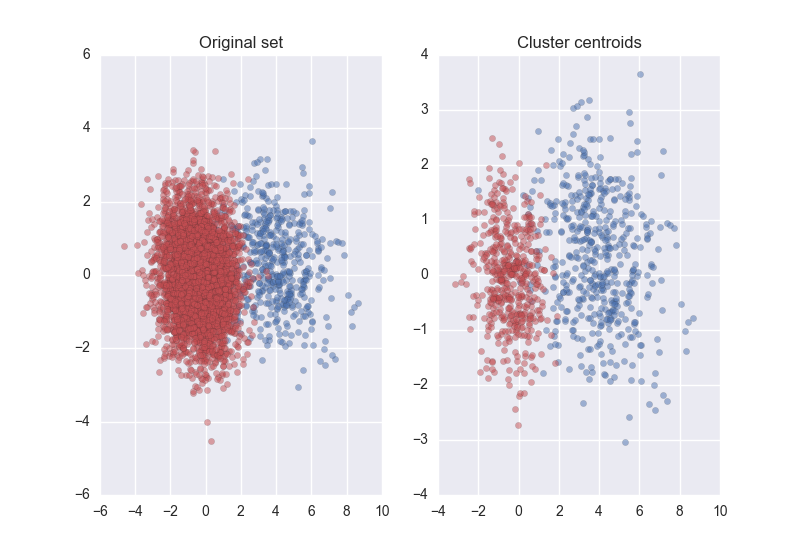
\includegraphics[width=0.3\linewidth]{sphx_glr_plot_cluster_centroids_001.png}} \hfill
%   \subfigure[]{\label{subfig:condensednearestneighbour}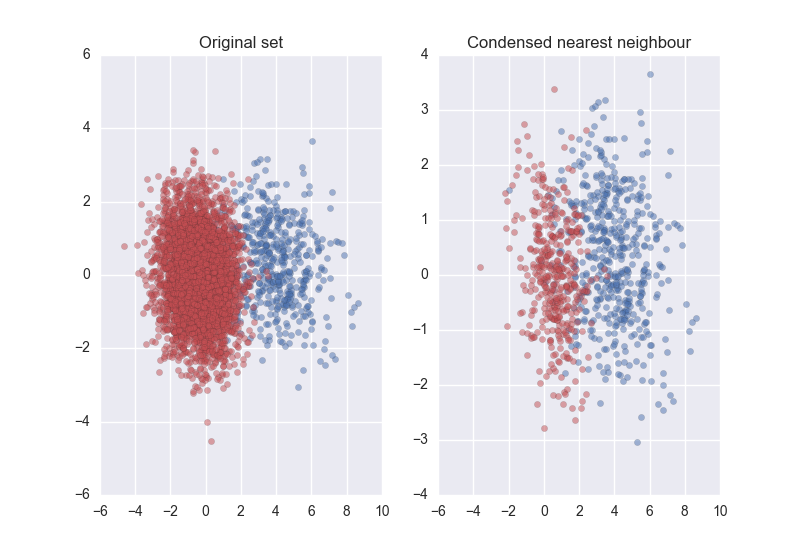
\includegraphics[width=0.3\linewidth]{sphx_glr_plot_condensed_nearest_neighbour_001.png}} \hfill
%   \subfigure[]{\label{subfig:editedneasrestneighbours}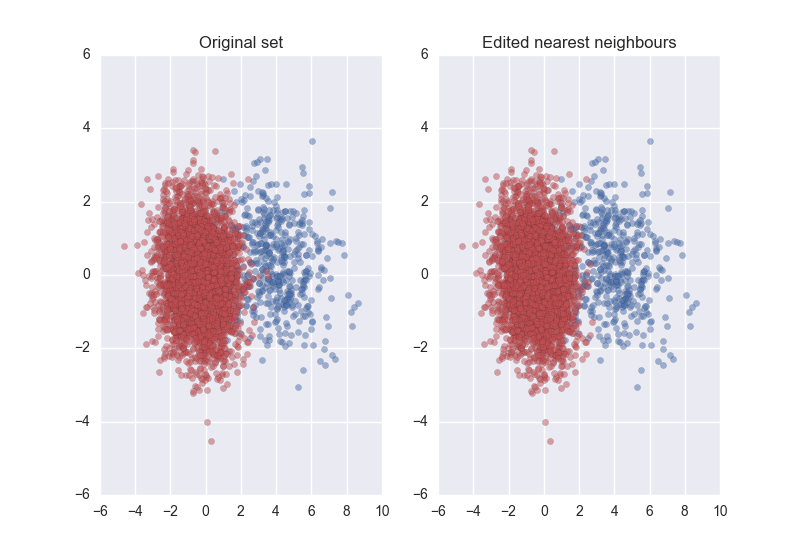
\includegraphics[width=0.3\linewidth]{sphx_glr_plot_edited_nearest_neighbours_001.png}}
%   \hspace*{\fill}\\
%   \hspace*{\fill}
%   \subfigure[]{\label{subfig:nearmiss1}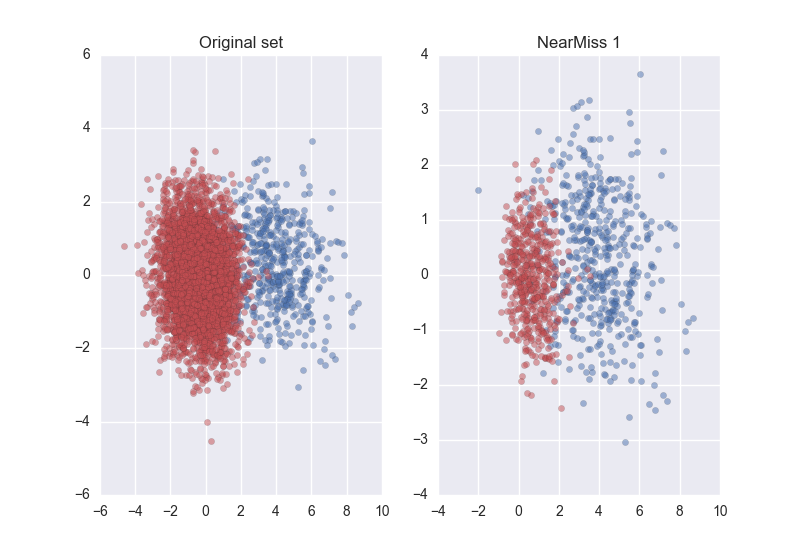
\includegraphics[width=0.3\linewidth]{sphx_glr_plot_nearmiss_1_001.png}} \hfill
%   \subfigure[]{\label{subfig:nearmiss2}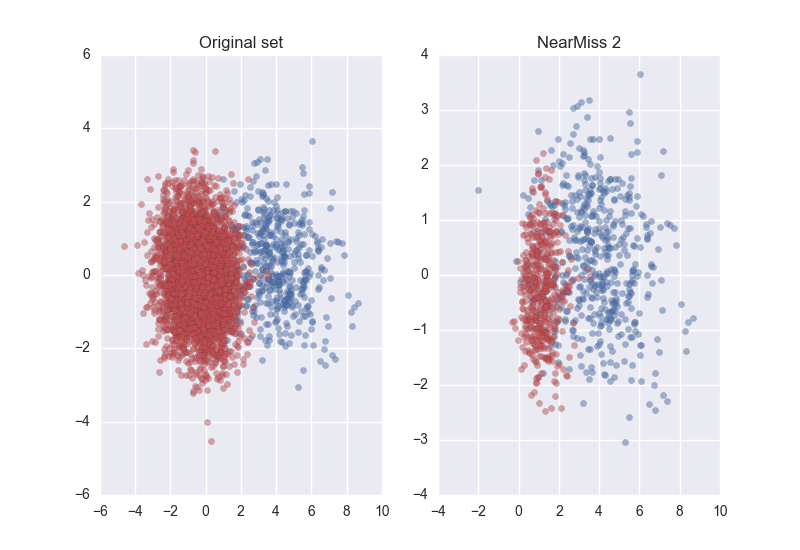
\includegraphics[width=0.3\linewidth]{sphx_glr_plot_nearmiss_2_001.png}} \hfill
%   \subfigure[]{\label{subfig:nearmiss3}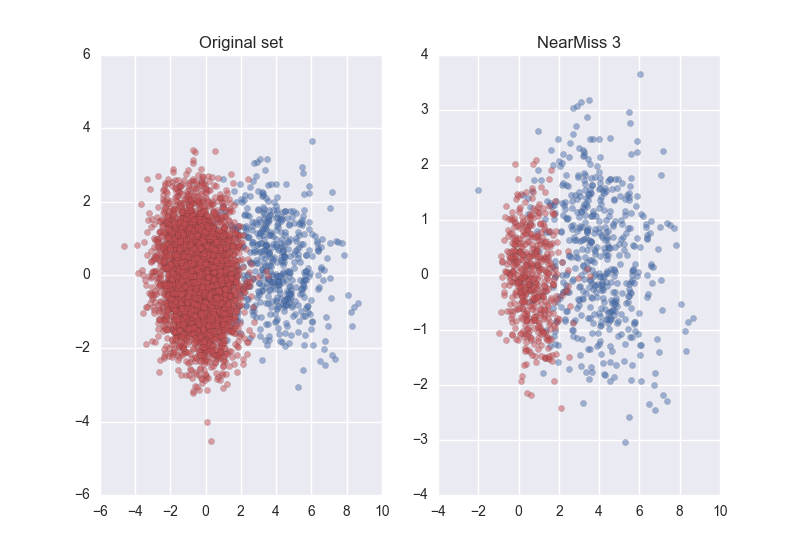
\includegraphics[width=0.3\linewidth]{sphx_glr_plot_nearmiss_3_001.png}}
%   \hspace*{\fill}\\
%   \hspace*{\fill}
%   \subfigure[]{\label{subfig:onesidedselection}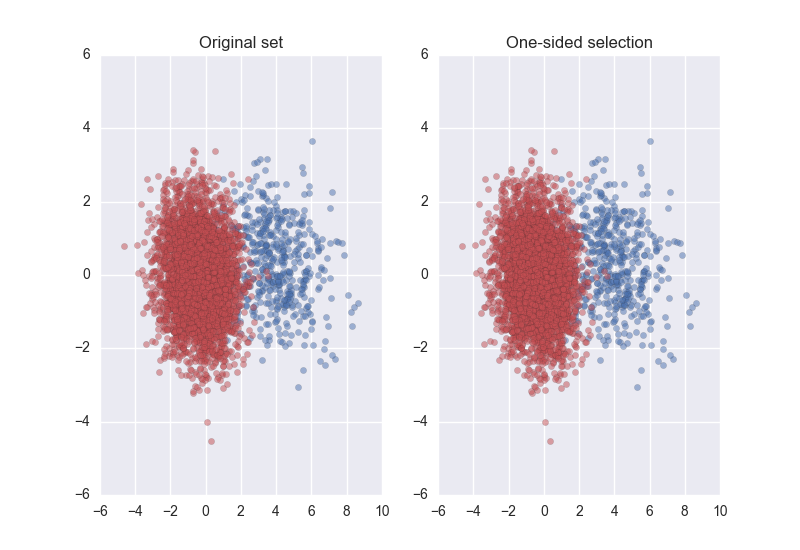
\includegraphics[width=0.3\linewidth]{sphx_glr_plot_one_sided_selection_001.png}} \hfill
%   \subfigure[]{\label{subfig:neighbourhoodcleaningrule}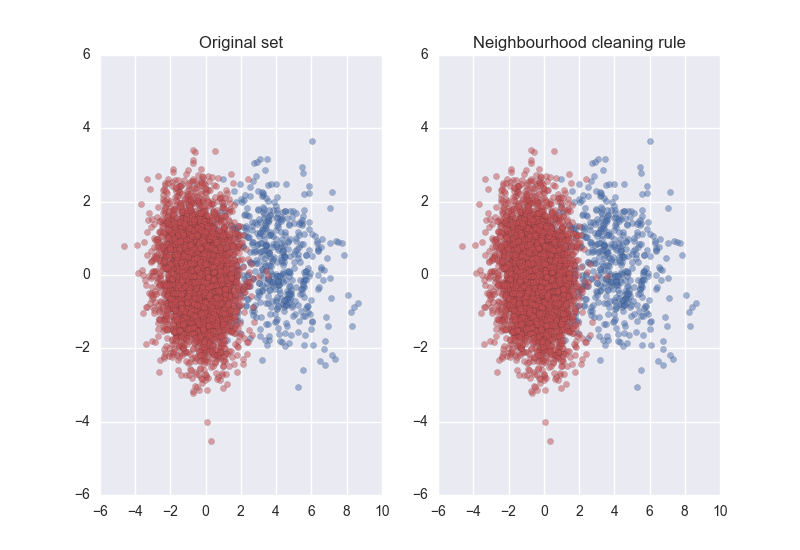
\includegraphics[width=0.3\linewidth]{sphx_glr_plot_neighbourhood_cleaning_rule_001.png}} \hfill
%   \subfigure[]{\label{subfig:tomeklinks}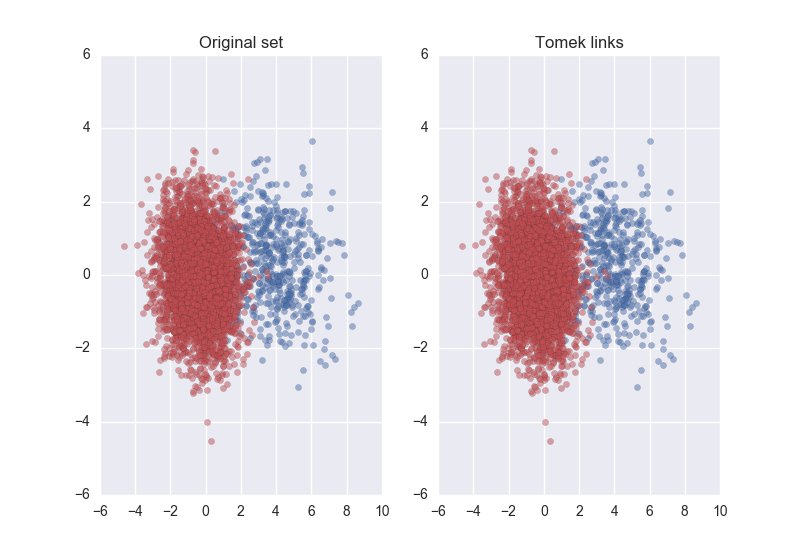
\includegraphics[width=0.3\linewidth]{sphx_glr_plot_tomek_links_001.png}}
%   \hspace*{\fill}\\
%   \hspace*{\fill}
%   \subfigure[]{\label{subfig:smote}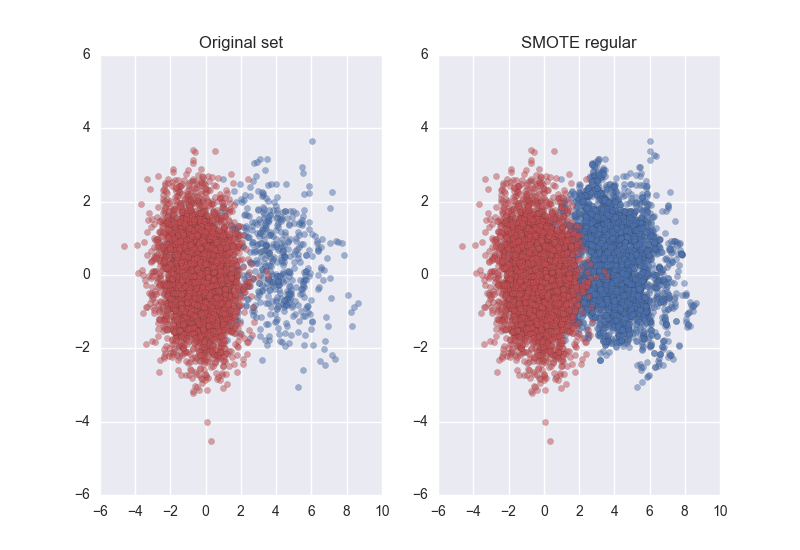
\includegraphics[width=0.3\linewidth]{sphx_glr_plot_smote_001.png}} \hfill
%   \subfigure[]{\label{subfig:smoteborderline1}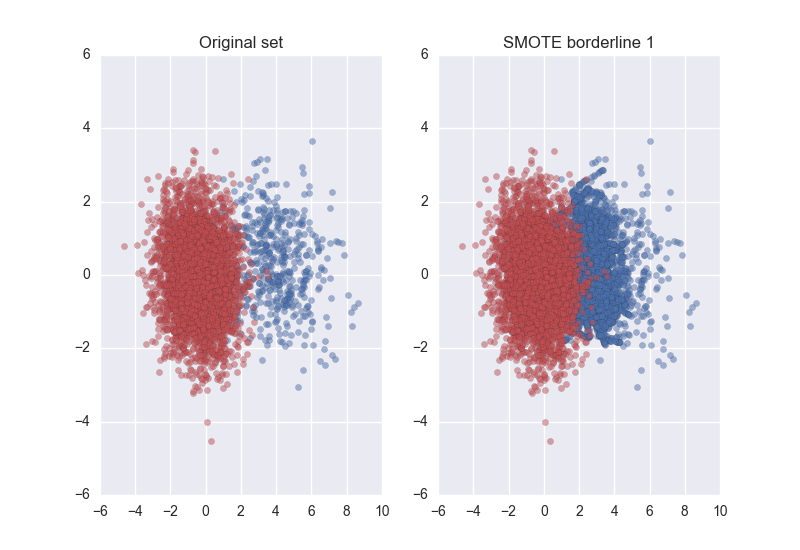
\includegraphics[width=0.3\linewidth]{sphx_glr_plot_smote_bordeline_1_001.png}} \hfill
%   \subfigure[]{\label{subfig:smoteborderline2}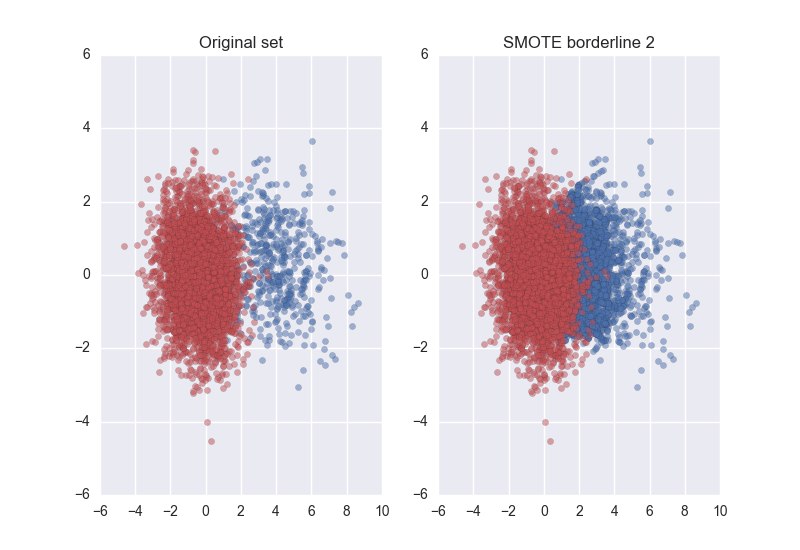
\includegraphics[width=0.3\linewidth]{sphx_glr_plot_smote_bordeline_2_001.png}}
%   \hspace*{\fill}\\
%   \hspace*{\fill}
%   \subfigure[]{\label{subfig:smotesvm}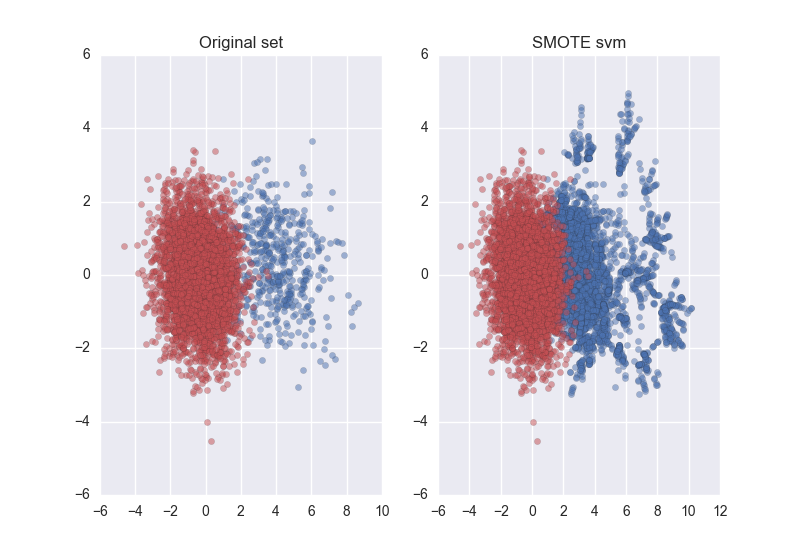
\includegraphics[width=0.3\linewidth]{sphx_glr_plot_smote_svm_001.png}} \hfill
%   \subfigure[]{\label{subfig:smoteenn}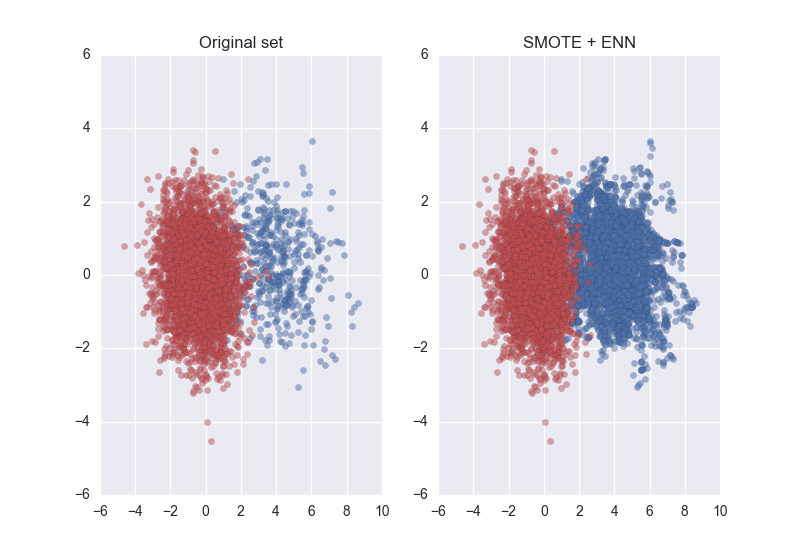
\includegraphics[width=0.3\linewidth]{sphx_glr_plot_smote_enn_001.png}} \hfill
%   \subfigure[]{\label{subfig:smotetomek}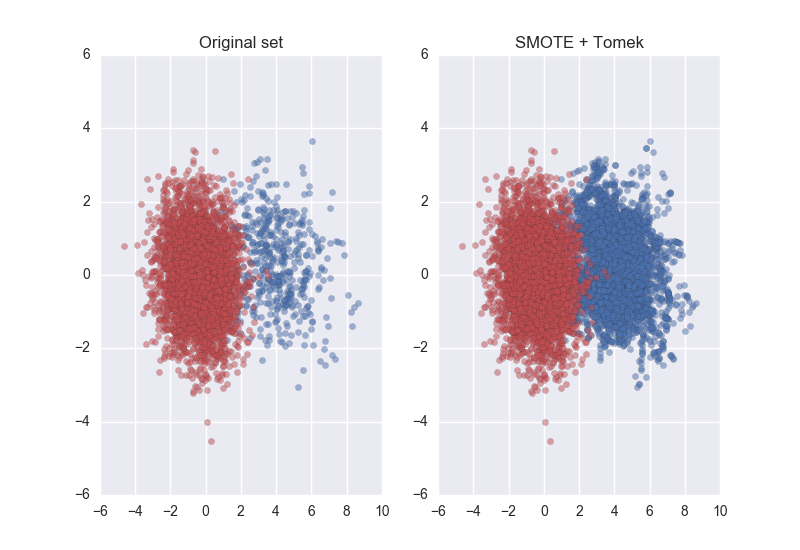
\includegraphics[width=0.3\linewidth]{sphx_glr_plot_smote_tomek_001.png}}
%   \hspace*{\fill}
%   \caption{Toy examples for the different sampling methods.}
%   \label{fig:methods}
% \end{figure}

\section{Conclusion}

In this paper, we shortly presented the foundations of the \texttt{UnbalancedDataset} toolbox vision and API.
As avenues for future work, the toolbox is intended to be fully part of a \texttt{scikit-learn-contrib} repository.

% \acks{We would like to acknowledge support for this project
% from git, GitHub, Travis CI, and Gitter.}

\bibliography{bibtex}


\end{document}
